\documentclass[a4paper, 11pt, twocolumn]{article}
\usepackage[utf8]{inputenc}
\usepackage{graphicx}
\usepackage[noend]{algorithm2e}
\usepackage{float}
\usepackage{amsmath}
\usepackage{amssymb}
\usepackage{epsfig,floatflt}
\usepackage{physics}
\usepackage[english]{babel}
\usepackage{booktabs}
\usepackage[round]{natbib}
%\usepackage{cite}
\usepackage[format=plain,
font=it]{caption}
\usepackage{url}
\usepackage{hyperref}
\usepackage{color}
\definecolor{darkred}{rgb}{0.5,0,0}
\definecolor{darkgreen}{rgb}{0,0.5,0}
\definecolor{darkblue}{rgb}{0,0,0.5}


\hypersetup{ colorlinks,
	linkcolor=darkblue,
	filecolor=darkgreen,
	urlcolor=darkred,
	citecolor=darkblue }

\usepackage{tikz}
\usetikzlibrary{matrix,positioning,decorations.pathreplacing,arrows}

\graphicspath{{../figures/}}
\DeclareGraphicsExtensions{.pdf}

\begin{document}

\title{Using Neural Networks and Logistic Regression for Classification and Regression Problems}

\author{Eina B. Jørgensen, Anna Lina P. Sjur and Jan-Adrian H. Kallmyr}

\twocolumn[
  \begin{@twocolumnfalse}
    \maketitle
    \begin{abstract}

We use a neural network (NN) and logistic regression (LR) to classify the 2005 Taiwan credit card data.
There are two categories: non-default and default. A comparison is made between
the two methods, and we find that the NN yields the highest accuracy score 0.823 compared with 0.820
from the LR algorithm.
Area under the receiver operating characteristic curve (AUC) was also used as a performance measure, the NN producing the highest score of 0.782, compared with 0.765 from logistic regression. The highest accuracy and AUC were found from different hyperparameters respectively. We also produced a confusion matrix, which showed that NN classified more true positives and true negatives correctly than LR.
In terms of efficiency, the LR algorithm converges quite rapidly compared to the NN, and is overall
more stable, possibly due to an implementation of dynamic learning rate.
Furthermore, we use the NN to fit the Franke function (with noise), and compare this to linear
regression algorithms used in our earlier paper. Our findings suggest that the neural
network achieved the lowest MSE of $0.011$, and a R2-score of $0.89$.

\end{abstract}

  \end{@twocolumnfalse}
]

\section{Introduction}
\label{sec:introduction}

% utkast til innledning
% kilde: ræva mi (trenger kilder)
The use of machine learning for problem solving has risen in popularity as large data sets have become available for analysis. There now exists many different methods in varying complexity for both supervised and unsupervised learning. All of these methods have advantages and drawbacks, as well as many similarities. This means that we can get familiar with some of the central themes in machine learning by studying simple algorithms, such as different linear regression schemes. A notable example is the bias-variance trade-off, where it is observed that the total mean-square-error (MSE) of a model starts off high, decreases until a minimum, and increases again (see Theory and Methods section.)

Starting with the Theory and methods section, we will describe three different algorithms for linear regression, as well as our resampling techniques and the bias-variance trade-off. In the Results section we will show our selected figures and data, with a focus on comparisons between the different methods. Moving on to the Discussion section we will consider the compared values and try to conclude which method seems to be most fit for fitting terrain data. We will also argue why that is the case. Finally, concluding in the Conclusion section, we will summarise the most important results as well as our thoughts around them.

\section{Theory and methods}
\label{sec:theory}

\subsection{Logistic Regression}
% Alt dette er henta fra lecture notes om logistisk regresjon, har bare ikke funnet riktig måte å referere ennå
Classification problems aim to predict the behaviour of a given object, and look for patterns based on discrete variables (i.e categories). Logistic regression can be used to solve such problems, commonly by the use of variables with binary outcomes such as true/false, positive/negative, success/failiure etc., or in the specific credit card case: \textit{risky/non-risky}

As opposed to linear regression, the equation one gets as a result of minimization of of the cost function by $\hat{\beta}$ using logistic regression, is non-linear, and is solved using minimization algorithms called \emph{gradient descent methods}. \\

When predicting the the output classes in which an object belongs, the prediction is based on the design matrix $\mathbf{\hat{X}} \in \mathbb{R}^{n\cross p}$ that contain $n$ samples that each carry $p$ features.

A distinction is made between \textit{hard classification} - deterministically determine the variable to a cathegory, and \textit{soft classification} - determines the probability that a given variable belongs in a certain cathegory. The latter is favorable in many cases, and logistic regression is the most used example og this type of classifier.

When using logistic regression, the probability that a given data point $x_i$ belongs in a cathegory $y_i$ is given by the Sigmoid-function (or logistic function):
\begin{equation}
\begin{split}
    & p(t) = \frac{1}{1 + e^{-t}} = \frac{e^t}{1+e^t} \\
    & 1-p(t) = p(-t)
\end{split}
  \label{eq:sigmoid}
\end{equation}

Assuming a binary classification problem, i.e. $y_i$ can be either 0 or 1, and a set of predictors $\hat{\beta}$ the Sigmoid function \eqref{eq:sigmoid} gives the probabilities with relation:
\begin{equation*}
  p(y_i = 0|x_i,\hat{\beta})  = 1 - p(y_i = 1|x_i,\hat{\beta})
  \label{eq:prob_relation}
\end{equation*}

The total likelihood for all possible outcomes $\mathcal{D}=\{(y_i,x_i)\}$ is used in the Maximum Likelihood Estimation (MLE), aiming at maximizing the log/likelihood funciton \eqref{eq:log_p}. The likelihood function can be expressed with $\mathcal{D}$:
\begin{equation*}
\begin{split}
    &\qquad P(\mathcal{D}|\hat{\beta}) = \\
    &\prod_{i=1}^n \qty[p(y_i = 1|x_i,\hat{\beta}) ]^{y_i}  \qty[1 - p(y_i = 0|x_i,\hat{\beta})]^{1-y_i}
\end{split}
\end{equation*}

And the log/likelihood function is then:
\begin{equation}
\begin{split}
    &P_{\log}(\hat{\beta}) = \\
    &\sum_{i=1}^n \Big(y_i \log \qty[p(y_i = 1|x_i,\hat{\beta})] \\
    &\quad+ (1-y_i) \log [1 - p(y_i = 0|x_i,\hat{\beta})]\Big)
\end{split}
\label{eq:log_p}
\end{equation}

The cost/error-function $\mathcal{C}$ (also called cross-entropy in statistics) is the negative of the log/likelihood. Maximizing $P_{\log}$ is thus the same as minimizing the cost function. The cost funciton is:
\begin{equation}
  \begin{split}
    &\mathcal{C}(\hat{\beta}) = - P_{\log}(\hat{\beta}) =  \\
    -&\sum_{i=1}^n \Big(y_i \log \qty[p(y_i = 1|x_i,\hat{\beta})] \\
    &\quad+ (1-y_i) \log [1 - p(y_i = 0|x_i,\hat{\beta})]\Big)
  \end{split}
  \label{eq:cost_function}
\end{equation}

Finding the parameters $\hat{\beta}$ that minimize the cost function is then done through derivation.
Defining the vector $\hat{y}$ containing $n$ elements $y_i$, the $n \cross p$ matrix $\hat{X}$ containing the $x_i$ elements, and the vector $\hat{p}$ that is the fittet probabilities $p(y_i|x_i,\hat{\beta})$, the first derivative of $\mathcal{C}$ is
\begin{equation}
  \nabla_\beta \mathcal{C} = \pdv{\mathcal{C}(\hat{\beta})}{\hat{\beta}} = - \hat{X}^T (\hat{y}-\hat{p})
  \label{eq:cost_d}
\end{equation}
This gives rise to set of linear equations, where the aim is to solve the system for $\hat{\beta}$.
By introduction of a diagonal matrix $\hat{W}$ with diagonal elements $p(y_i|x_i,\hat{\beta})\cdot(1-p(y_i|x_i,\hat{\beta}))$ the second derivative is:
\begin{equation}
 \pdv[2]{\mathcal{C}(\hat{\beta})}{\hat{\beta}}{\hat{\beta}^T} = \hat{X}^T\hat{W}\hat{X}
 \label{eq:cost_dd}
\end{equation}

With $\hat{x} = [1, x_1,x_2,...,x_p]$ and $p$ predictors $\hat{\beta} = [\beta_0,\beta_1,\beta_2,...,\beta_p]$ the ration between likelihoods of outcome is:
\begin{equation}
  \log \frac{p(\hat{\beta}\hat{x})}{1-p(\hat{\beta}\hat{x})} = \beta_0 + \beta_1x_1 + ... + \beta_px_p
  \label{eq:prob_ratio}
\end{equation}

\noindent and $p(\hat{\beta}\hat{x})$ defined by:
\begin{equation}
  p(\hat{\beta}\hat{x}) = \frac{e^{\beta_0 + \beta_1x_1 + ... + \beta_px_p}}{1+e^{\beta_0 + \beta_1x_1 + ... + \beta_px_p}}
  \label{eq:pBx}
\end{equation}

\subsection{Gradient Descent Methods}
\subsubsection*{The General Idea}
With the gradient of $\mathcal{C}$ defined as in \eqref{eq:cost_d}, we use this to find the minimum of the cost function. The basic idea is that by moving in the direction of the negative gradient of a function, we can move towards the value (in this case the $\beta$) that minimizes the function (in this case $\mathcal{C}(\beta)$)

This is done by repeating the algorithm
\begin{equation}
    \beta_{j+1} = \beta_j - \gamma \nabla_\beta \mathcal{C}(\beta) \quad j = 0,1,2,...
    \label{eq:gradient_decent}
\end{equation}
When a minimum is approached, $\nabla_\beta \mathcal{C}(\beta) \rightarrow$ 0, and thus we can set a limit when $\beta_{k+1} \approx \beta_k$ given a certain tolerance, and the $\beta$ which minimizes the cost funciton is found. $\gamma$ is in this case called the \textit{learning rate}, and is a parameter that must be tuned to each specific case in order to optimize the regression.

\subsubsection*{Stochastic Gradient Descent}
In this project we use a stochastic version of gradient descent, which is an improvement upon the regular gradient descent (HOW??). This is done by expression the cost function (and thus also its gradient) as a sum
\begin{equation}
    \nabla_\beta \mathcal{C}(\beta) = \sum_i^n     \nabla_\beta c_i(\boldsymbol{x_i},\beta) ,
    \label{eq:gradient_sum}
\end{equation}
and by only taking calculating the gradient of a subset of the data at the time. These subsets, called \textit{minibatches} are of size $\boldsymbol{M}$ , and the total amount is $\frac{n}{\boldsymbol{M}}$ where $n$ is the amount of data points. The minibatches are denoted $\boldsymbol{B}_k$, with k = 1,2,...,$\frac{n}{\boldsymbol{M}}$.

Instead of a sum over all the the data points $i \in [1,n]$ we now in each step, sum over all the data points in the given minibatch $i \in \boldsymbol{B}_k$ where $k$ is picked randomly with uniform proabaility from $[1, \frac{n}{\boldsymbol{M}}]$.

The stochastic and final version of \eqref{eq:gradient_decent} is therefore given by the algorithm

\begin{equation}
    \beta_{j+1} = \beta_j - \gamma_j \sum_{i \in \boldsymbol{B}_k}\nabla_\beta c_i(\boldsymbol{x_i},\beta)
    \label{eq:stochstic_gradient_descent}
\end{equation}
An iteration over the total number of minibatches is commonly refered to as an \textit{epoch.}\\

By using the stochastic gradient descent method \eqref{eq:stochstic_gradient_descent} to minimize the cost function \eqref{eq:cost_function} we can this find the $\beta$ values that give the most accurate classification, by doing \textit{logistic regression}.

\subsection{Neural networks} 
In this section, the equations used are based off the book by \cite{Nielsen}.
\subsubsection*{The structure of a network}
Neural networks, as the name suggests, are inspired by our understanding of how networks of neurons function in the brain. As can be seen in the example network in Figure \ref{fig:NNstructure}, neurons are structured in layers. We always have a input and an output layer, in addition to a varying number of hidden layers. The input layer has as many neurons as there are input variables, while the output layer has one neuron for each output. How many neurons you have in the output layer depends on the specific problem. The number of neurons in each hidden layer, on the other hand, is not directly related to inputs or outputs, and must be decided in some other way.

As the diagram in Figure \ref{fig:NNstructure} suggests, the neurons in each layer are not connected with each other, but takes in inputs from the previous layer and passes on an output to the neurons in the next layer, as illustrated with arrows. This way, the inputs are fed through the network and processed, resulting in an output.
\begin{figure}[htbp]
	\centering
	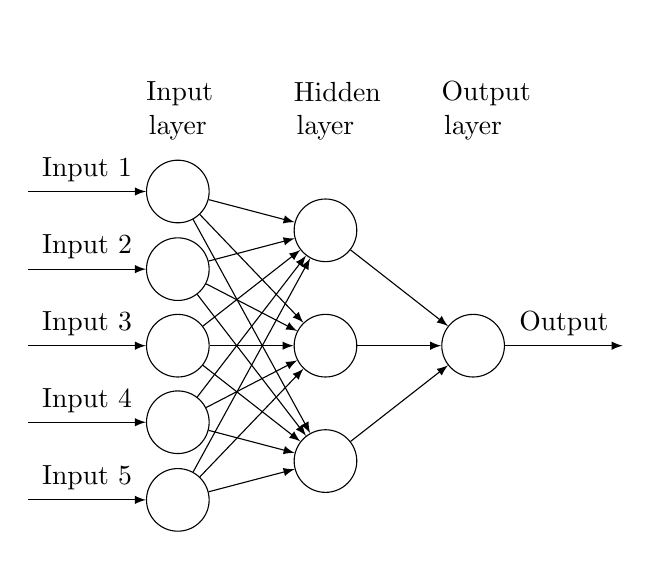
\begin{tikzpicture}[
	plain/.style={
		draw=none,
		fill=none,
	},
	net/.style={
		matrix of nodes,
		nodes={
			draw,
			circle,
			inner sep=8pt
		},
		nodes in empty cells,
		column sep=0cm,
		row sep=-9pt
	},
	>=latex
	]
	\matrix[net] (mat)
	{
		|[plain]| \parbox{0.8cm}{\centering Input\\layer} & |[plain]| \parbox{0.8cm}{\centering Hidden\\layer} & |[plain]| \parbox{0.8cm}{\centering Output\\layer} \\
		& |[plain]| \\
		|[plain]| & \\
		& |[plain]| \\
		|[plain]| & |[plain]| \\
		& & \\
		|[plain]| & |[plain]| \\
		& |[plain]| \\
		|[plain]| & \\
		& |[plain]| \\    };
	\foreach \ai [count=\mi ]in {2,4,...,10}
	\draw[<-] (mat-\ai-1) -- node[above] {Input \mi} +(-1.9cm,0);
	\foreach \ai in {2,4,...,10}
	{\foreach \aii in {3,6,9}
		\draw[->] (mat-\ai-1) -- (mat-\aii-2);
	}
	\foreach \ai in {3,6,9}
	\draw[->] (mat-\ai-2) -- (mat-6-3);
	\draw[->] (mat-6-3) -- node[above] {Output} +(1.9cm,0);
	\label{fig:NNstructure}
	\end{tikzpicture}
	\caption{Schematic diagram of a neural network with five input neurons in the input layer, one hidden layer with tree neurons and a single output neuron in the output layer.}
	\label{fig:NNstructure}
\end{figure}

\subsubsection*{Forward feeding}
Each neuron has one or multiple inputs, as illustrated with arrows in Figure \ref{fig:NNstructure}. Each of these inputs has a weight associated with it. To clarify the notation used, let's take a look at the $j$th neuron in the $l$th layer. The weight associated with the input coming from the $k$th neuron in the previous layer is denoted as $w^l_{jk}$. In addition, each neuron has a bias associated with it, for the neuron in question denoted as $b^l_j$. Summing the weighted inputs and the bias, and feeding this to a function $\sigma$, gives the activation $a^l_j$:
\begin{equation*}
	a^l_j = \sigma\left(\left(\sum_{k}w^l_{jk}a^{l-1}_k\right) + b^l_j\right)
\end{equation*}
This activation is then fed forward as input to all the neuron in the next layer.

In matrix notation, the activation for the whole layer $l$ can be written as
\begin{equation}\label{eq:forward}
	\boldsymbol{a}^l = \sigma\left(\boldsymbol{w}^l\boldsymbol{a}^{l-1}+\boldsymbol{b}^l\right)
\end{equation}
Here, $\boldsymbol{a}^l$ and $\boldsymbol{b}^l$ are vertical vectors containing the activations and biases of the $l$th layer, while $\boldsymbol{w}^l$ is a matrix with elements $w^l_{jk}$, i.e. the $j$th column contains the weights of the inputs reaching the $j$th neuron.  

Let's look at the activation function in Eq. (\ref{eq:forward}) denoted with a $\sigma$. The use of $\sigma$ as notation is not arbitrary, since the sigmoid function stated in Eq. (\ref{eq:sigmoid}) is often used. As we will see in the backpropagation algorithm, the sigmoid is a good choice for activation function, since a small change in the output can be propagated backwards, resulting in small changes in the weights and biases through the network.


With a basis in Eq. (\ref{eq:forward}), the algorithm for forward feeding is given in Algorithm \ref{alg:forward}. Here $L$ is the total number of layers. 
\begin{algorithm}[htbp]\caption{The forward feeding algorithm.}\label{alg:forward}
	\SetAlgoLined
	\BlankLine
	\BlankLine
	Set $\boldsymbol{a}^1$ = input\;
	\ForEach{l=2:L}{
		Compute  $\boldsymbol{a}^l$\;}
	Set output to $\boldsymbol{a}^L$\;
	\BlankLine
	\BlankLine
\end{algorithm}

Note that the output will have values between 0 and 1, when the sigmoid function is used to compute the activations of all the layers. In a classification problem, this corresponds to the likelihood of an outcome. For example, in a classification problem with five classes, the network would have five output neurons, each representing a class. The final classification of an input would then be the class with the highest probability. 

\subsubsection*{Backpropagation}
When training the network, the goal is to find the weights and biases that minimize the cost function $C$. For a classification problem, the cost function is often given as

\begin{equation}\label{eq:costNN}
	C = \frac{1}{2}\sum_{i}\left(a^L_i-y_i\right)^2
\end{equation}  
To minimize Eq.(\ref{eq:costNN}), one can use Stochastic Gradient Decent, as described previously. But in order to use SGD, the derivatives of $C$ must be computed, and it is here that backpropagation comes in. It can be shown that the derivatives are given as in Eq. (\ref{eq:backprop}). For a derivation of these expressions see APPENDIX?!?!?!. 

\begin{equation}\label{eq:backprop}
\begin{aligned}
	\delta^L &= \nabla_aC\odot\sigma'(z^L)\delta^l \\ 
	\delta^l &= ((\boldsymbol{w}^{l+1})^T\delta^{l+1})\odot\sigma'(\boldsymbol{z}^l) \\
	\frac{\partial C}{\partial b^l_j} &= \delta_j^l \\
	\frac{\partial C}{\partial w_{jk}^l} &= a_k^{l-1}\delta^l_j
\end{aligned}
\end{equation}
These equation are the basis for the backpropagating algorithm, described in Algorithm \ref{alg:backprop}. 
\begin{algorithm}[htbp]\caption{The backpropagation algorithm.}\label{alg:backprop}
	\SetAlgoLined
	\BlankLine
	\BlankLine
	Compute $\{ \boldsymbol{a}^l\}_{l=1}^L$ with feed forward\;
	Compute $\delta^L$\;
	Set $\frac{\partial C}{\partial \boldsymbol{b}^L} = \delta^L$\;
	Compute $\frac{\partial C}{\partial \boldsymbol{w}^L} = \delta^L(\boldsymbol{a}^{L-1})^T$\;
	\ForEach{l=L-1:2}{
		Compute $\delta^l$\;
		Set $\frac{\partial C}{\partial \boldsymbol{b}^l} = \delta^l$\;
		Compute $\frac{\partial C}{\partial \boldsymbol{w}^l} = \delta^l(\boldsymbol{a}^{l-1})^T$\;
	}
	\BlankLine
	\BlankLine
	\end{algorithm}
	
\subsubsection*{Adapting neural networks to regression}
In order to adapt the network to regression, some changes must be made in Algorithm \ref{alg:forward} and \ref{alg:backprop}.  

\subsubsection*{Implementation}


\subsection{Data sets}
In this report, the default of credit card clients data set \citep{yeh2009UCI} was used to study the performance and compare the logistic regression method and neural networks. A description of the attributes of the data set can be found in \cite{yeh2009UCI}. Upon inspection, it is notable that the data set contains a considerable amount of values different from their valid values as described by \citeauthor{yeh2009UCI}. Mostly, this apply for the categorical variables, where the given value does not correspond to any category. By removing data points with invalid values, as well as entries where the client does not have any history of past payments or bill statements, the data set is reduced from 30000 data points to 3792 points. As this is a considerable reduction of data points, a second reduced data set was constructed, where OGSÅ HVA VI GJORDE

In addition the default of credit card clients data set, data produced with Franke's function was applied to neural networks. For details on Frnake's function, see \cite{prosjekt1}. 


\section{Results}
\label{sec:results}

\subsection{Diffusion equation}

In Figure \ref{fig:FDcompare} two different instants in the time evolution of the diffusion equation (eq. \ref{eq:diffusionEQ}), as obtained from finite difference methods, are shown. For both, a comparison is made with the exact solution and a run with higher spatial resolution ($\Delta x = 1/100$) and lower spatial resolution ($\Delta x = 1/10$). In both cases, the graphs of the exact solution and the one with higher spatial resolution are difficult to distinguish.
 \begin{figure}[htbp]
  	\centering
  	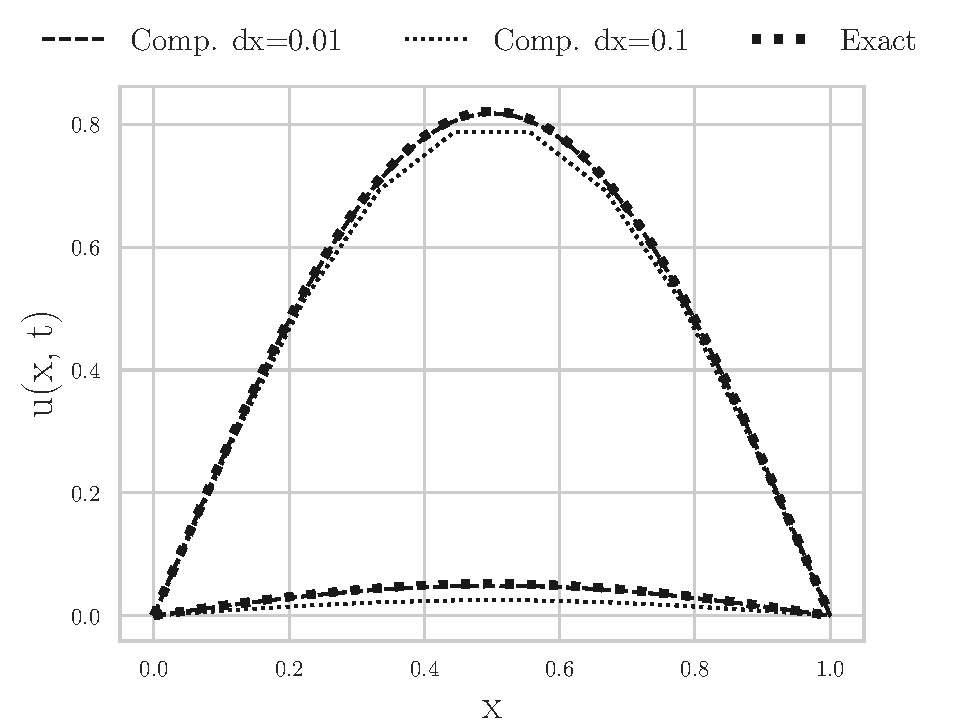
\includegraphics[width=0.5\textwidth]{FD_solved_new}
  	\caption{Time evolution of eq. \ref{eq:diffusionEQ} solved using finite difference methods: CD and FE for time's $t=0.02$ s and $t=0.3$ s. For each point in time a visual comparison is made with the exact solution.}
   \label{fig:FDcompare}
 \end{figure}

Likewise, in Figure \ref{fig:NNcompare} we show a parallell to Figure \ref{fig:FDcompare} with solutions from a neural network. In this case, we also see agreement between the computed and exact solutions for both points in time.
 \begin{figure}[htbp]
  	\centering
  	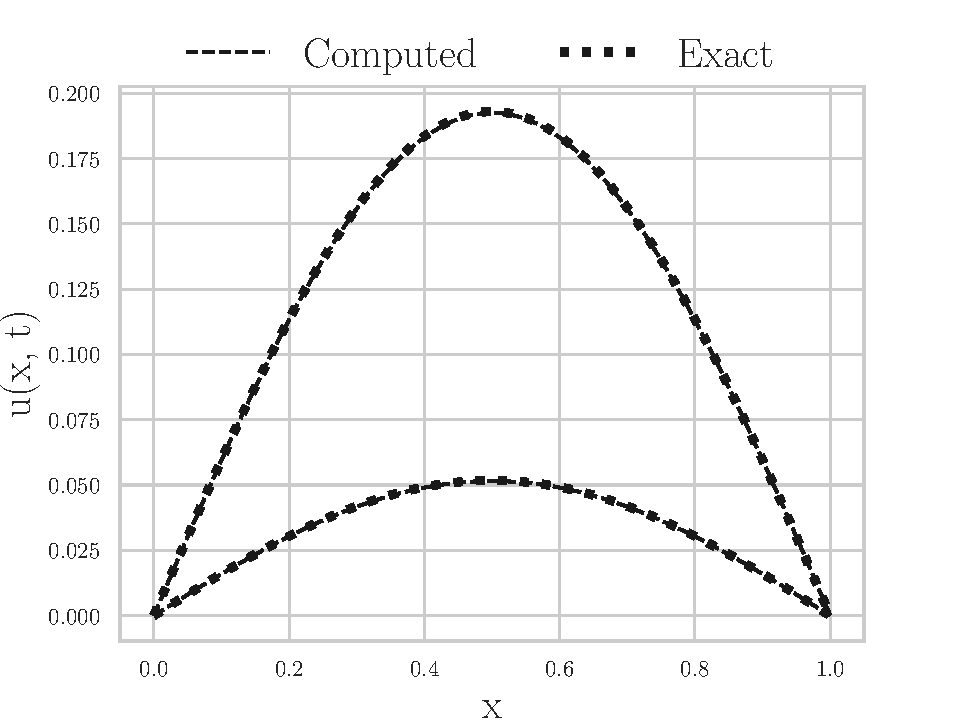
\includegraphics[width=0.5\textwidth]{NN_solved}
  	\caption{Time evolution of eq. \ref{eq:diffusionEQ} solved using a neural network. For both instants in time, $t=0.02$ s and $t=0.3$ s, a visual comparison is made with the exact solution, represented by dotted lines. The computations are done with $N_t = 30$ and $N_x = 100$.}
   \label{fig:NNcompare}
 \end{figure}

Shown in Figure \ref{fig:MSEbench} are the MSE's for two instants in time for both finite difference methods and a neural network. For the finite difference methods we observe a decrease in MSE for increasing temporal solution, slowing down after around 500 time points for both cases. For $t=0.02$ s (a.), the MSE is minimal at around $10^{-6}$ for 1000 time points, while for $t=0.3$ s (c.) it only becomes around $10^{-5}$ for 1000 time points.

For the neural network, we observe a decrease in MSE for an increasing number of iterations. In the case of $t=0.02$ s (b.), we see that the MSE decreases below $10^{-8}$ after around 6000 iterations, with a further, but slight, decrease at 10000 iterations. As for $t=0.3$ s (d.), the MSE is below $10^{-8}$ after around 4000 iterations and is mostly unchanged afterwards.

Comparison between the finite difference methods and the neural network, we see that the neural network can obtain an MSE 2-3 orders of magnitude lower than the finite difference methods.
\begin{figure}[htbp]
 	\centering
 	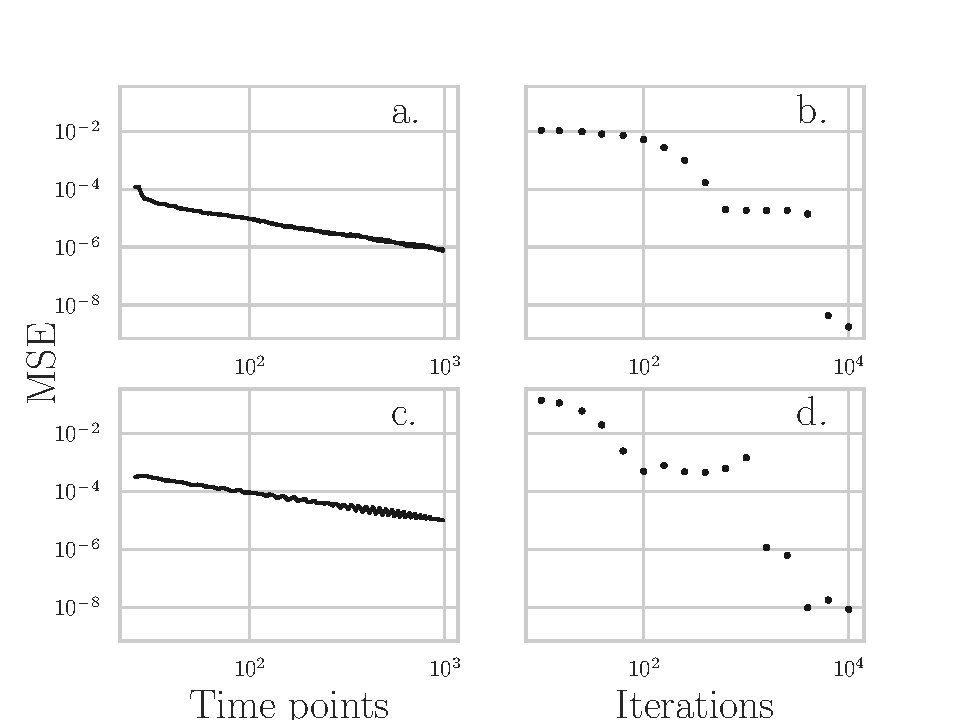
\includegraphics[width=0.5\textwidth]{MSEbench}
  \caption{Shown on the left-hand side, top-to-bottom (a., c.), are the MSE's as a function of temporal resolution, obtained from using finite difference methods for $t=0.02$ and $t=0.3$, respectively. Likewise, on the right-hand side (b., d.) the MSE's yielded from the neural network are shown as a function of iterations with network parameters $N_t = 10$, $N_x = 100$, and $\gamma = 0.004$.}
  \label{fig:MSEbench}
\end{figure}

Accompanying Figure \ref{fig:MSEbench}, we show the CPU times as a function of temporal resolution and number of iterations, respectively, for the different scenarios in Figure \ref{fig:CPUbench}. We see that the general curve is very similar for all scenarios. For the CD/FE method, we see that the CPU time becomes slightly longer for shorter t at 1000 time points. The neural network looks to have the same curve in both b. and d.

Comparing the two methods, we see that the neural network is around 3 orders of magnitude, if not more, slower than the finite difference methods.
\begin{figure}[htbp]
 	\centering
 	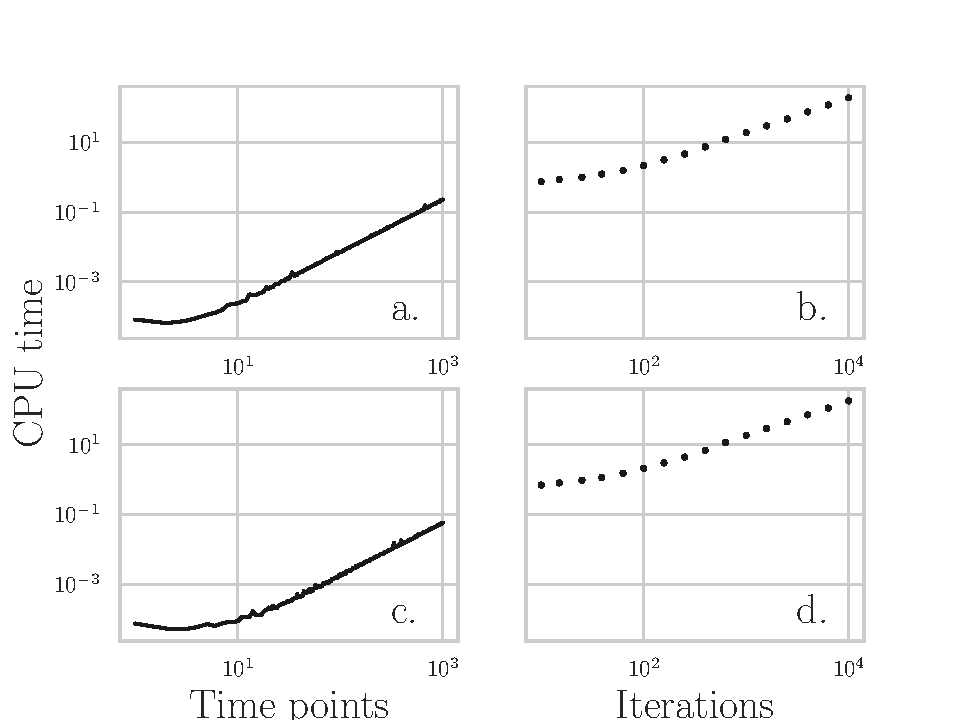
\includegraphics[width=0.5\textwidth]{CPUbench}
 	\caption{Shown on the left-hand side, top-to-bottom (a., c.), are the CPU time's as a function of temporal resolution, obtained from using finite difference methods for $t=0.02$ and $t=0.3$, respectively. Likewise, on the right-hand side (b., d.) the CPU time's yielded from the neural network are shown as a function of iterations with network parameters $N_t = 10$, $N_x = 100$, and $\gamma = 0.004$.}
  \label{fig:CPUbench}
\end{figure}


\subsection{Eigenpairs}
Looking at the eigenpairs of matrix A (\ref{matrix:A}), the maximum eigenvalue computed with  \texttt{numpy.linalg} is given under as $w_{max}^{np}$, with corresponding eigenvector $v_{max}^{np}$. The same eigenpair, computed with a neural network, is given as $w_{max}^{nn}$ and $v_{max}^{nn}$. Note that the eigenvectors have been normalized, to allow for comparison. We see that the two eigenvalues only differ at the 5th decimal place, while the eigenvector elements first differ at the 3th decimal place. Comparing the CPU times of the two methods for one run, the neural network is slower by a factor of about 1000.  

\begin{equation*}
v_{max}^{np} = \begin{bmatrix}
	0.4025950 \\
	0.4790814 \\
	0.3357358 \\
    0.3835011 \\
    0.3542414 \\
    0.4723555
\end{bmatrix} \quad w_{max}^{np} =  2.83515
\end{equation*}

\begin{equation*}
v_{max}^{nn} = \begin{bmatrix}
	0.40165637 \\
	0.47992723 \\
	0.33576365 \\
	0.38384145 \\
	0.35298366 \\
	0.47294087
\end{bmatrix} \quad w_{max}^{nn} = 2.83514
\end{equation*}

How $v_{max}^{nn}$ evolves over time is shown in Figure \ref{fig:eigenvector_max}. The network used for this computation had three hidden layers, all with ten neurons. The learning rate was 0.001, while the time step was 0.1. The precision, which was the MSE at which the training was stopped, was set to $10^{-4}$, resulting in 10820 iterations. 

 \begin{figure}[htbp]
 	\centering
 	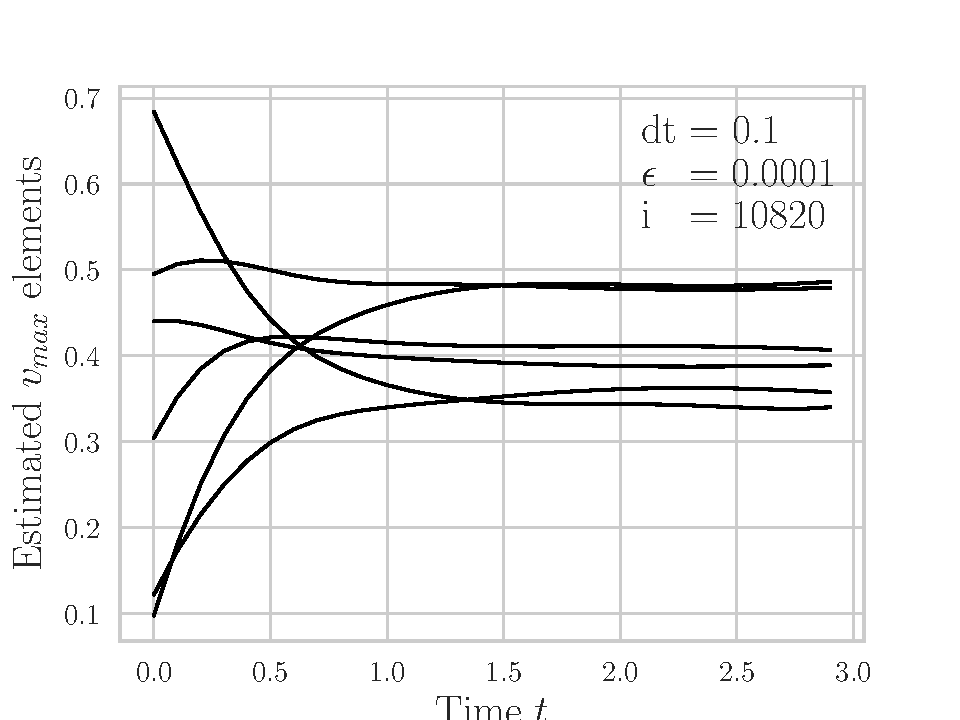
\includegraphics[width=0.5\textwidth]{eigenvector_max}
 	\caption{Figure showing how the value of the elements of the estimated eigenvector $v_{max}$ evolves over time, when computed by a neural network. Each line represents one of the elements of the vector. Time step $dt$, precision $\epsilon$ and iterations $i$ needed to achieve that precision is also shown.}
 	\label{fig:eigenvector_max}
 \end{figure}
 
 Analogously to what was shown above for the maximum eigenvalue, the minimum eigenvalue computed with \texttt{numpy.linalg} is shown below as $w_{min}^{np}$ together with the corresponding eigenvector $v_{min}^{np}$. Similarly, the same pair computed with neural network is denoted as $w_{min}^{nn}$ and $v_{min}^{nn}$. Again, the eigenvalues differ first at the 5th decimal place, and the egenvectors differ at the 3th decimal place, not taking the sign into account. 

\begin{equation*}
  v_{min}^{np} = \begin{bmatrix}
   0.6928048 \\
  -0.0074343 \\
  -0.7048516 \\
  -0.1487365 \\
  0.0122096 \\
  0.0296413
  \end{bmatrix} \quad w_{min}^{np} = -0.515594
\end{equation*}

\begin{equation*}
  v_{min}^{nn} = \begin{bmatrix}
   -0.69116113  \\
   0.00492352  \\
   0.70646873  \\
   0.14887754 \\
   -0.01982836 \\
   -0.02482513
  \end{bmatrix} \quad w_{min}^{nn} = -0.515528
\end{equation*}

Similarly to Figure \ref{fig:eigenvector_max}, the graph in Figure \ref{fig:eigenvector_min} shows the evolution of the eigenvector $v_{min}^{nn}$. Note the different time values in the two figures. The same network, with the same configurations as described above, is used, except that $A$ was replaced with $-A$ in the cost function. To reach a precision of $10^{-4}$, 842653 iterations was needed. 

\begin{figure}[htbp]
 \centering
 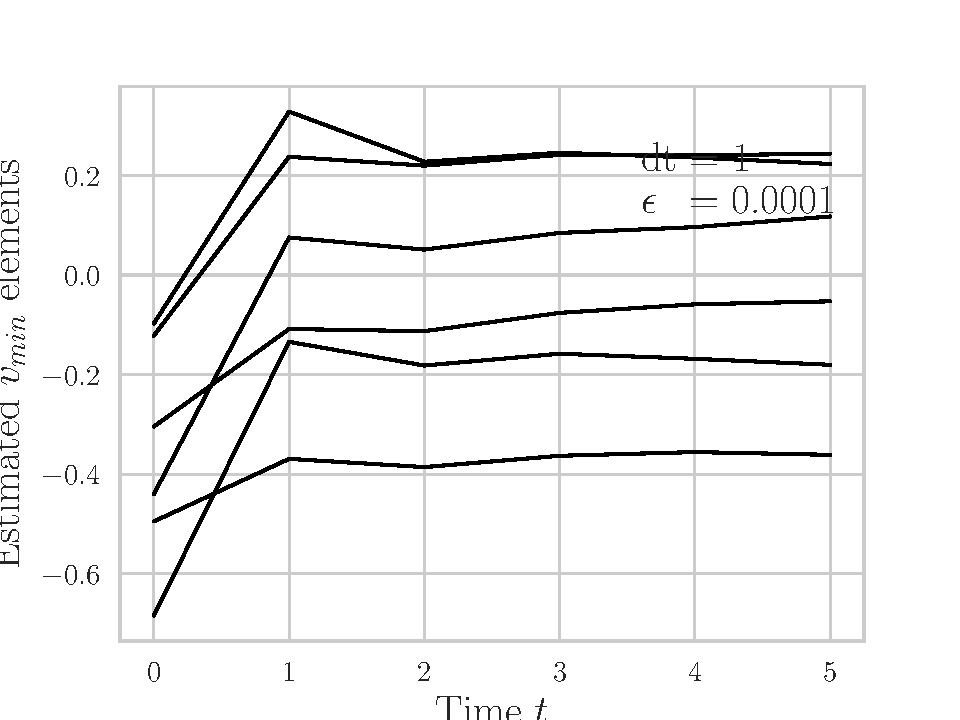
\includegraphics[width=0.5\textwidth]{eigenvector_min}
 \caption{Figure showing how the value of the elements of the estimated eigenvector $v_{min}$ evolves over time, when computed by a neural network. Each line represents one of the elements of the vector. Time step $dt$, precision $\epsilon$ and iterations $i$ needed to achieve that precision is also shown.}
 \label{fig:eigenvector_min}
\end{figure}

% Eksempel for figurer
% \begin{figure}[htbp]
% 	\centering
% 	\includegraphics[width=0.5\textwidth]{}
% 	\caption{}
% 	\label{fig:}
% \end{figure}


\section{Discussion}
\label{sec:discussion}

% Discuss beta confidence intervals
\subsubsection*{Behaviour of the different regression methods applied to Franke's function}
Let's first look at the $\boldsymbol{\beta}$ confidence interval in Figure \ref{fig:biasvarianceOLS}. As we can see, the range of values that has a 95\% probability of containing $\beta_i$ is quite wide, for some in the same order of magnitude as the $\beta$-value itself. Considering the expression for the interval, stated in (\ref{eq:confidence}), we see that the width of the interval strongly depends on the spread of $\boldsymbol{\epsilon}$ in (\ref{eq_model}). As the noise term $\boldsymbol{\epsilon}$ goes to zero, so does the width of the confidence interval.

% Discuss R2 and MSE values for the different methods
Looking at the  the mean squared error and the $R^2$-value of the approximation to Franke's function using ordinary least squares (Figure \ref{fig:mseVSdegreeOLS} and \ref{fig:r2VSdegreeOLS}), we see the difference in the results when using the entire training set as test data, and when separating the data into test and training data using resampling. Comparing the two results, they both display the same trend: When train and test data is not separated, the approximation seems to unambiguously become better with increased model complexity, though, converging to what looks to be the minimum error. When using designated test data, however, it becomes apparent that using the training data for testing gives a false sense of security, as the mean squared error now starts increasing and the $R^2$-value decreasing when a certain model complexity is reached. It appears that a complexity given by a polynomial of degree $m \in [5,7]$ gives the best result for both the $R^2$-value and the MSE when using OLS in this case.

From equation \eqref{eq:bias-variance} we expect the total error to be the sum of the bias squared, the variance of model, plus some irreducible error. Looking at Figure \ref{fig:biasvarianceOLS}, showing the MSE, variance and bias for the ordinary least squared method on Franke's function, we see that the results displayed correspond nicely with these expectations. Thus we observe how bias and variance gives rise to the shape of the MSE curve, both in Figure \ref{fig:biasvarianceOLS} and \ref{fig:mseVSdegreeOLS}. As discussed in lectures, and explained in \cite{hastie2009elements}, a higher variance for a more complex polynomial is a consequence of over fitting, allowing the polynomials to fit to the noise in the data. When only using the training data as test data, this over fitting goes unnoticed, which is the reason for the behaviour of the training data curve in Figure \ref{fig:mseVSdegreeOLS}.

Understanding the importance of proper use of test data and resampling, we move on to compare the now discussed ordinary least squares method to our two other regression methods, Ridge regression and Lasso regression. We have here, as can be seen in Figure \ref{fig:lambdavsdegreesRIDGE} and \ref{fig:lambdavsdegreesLASSO}, chosen to focus on comparing the MSE of the methods, as opposed to the $R^2$-score simply because we found it more intuitive.

Moving into the territory of regression methods with hyperparameters, we study the behaviour of the mean squared error of the approximations for various values of $\lambda$ and varying complexity.
Common for both Lasso and Ridge is the almost constant behaviour of the MSE after reaching a certain model complexity, even when a designated test set is used. This stands in contrast to the convex shape of the OLS-MSE in Figure \ref{fig:mseVSdegreeOLS}. By adding the penalty term in (\ref{eq:ridge_cost}) and (\ref{eq:lasso}), we introduce a bias to the model. However, the penalty term also prevents over-fitting, and thus reduces the model variance.

Focusing on the behaviour of the MSE for different tuning parameters $\lambda$, it appears that the model preforms better for smaller $\lambda$.

Looking at the minimum MSE values of both Ridge and Lasso, the first preforms somewhat better than the latter on Franke's function. Both OLS and Ridge reaches a minimum MSE of about 0.015, with Ridge performing slightly better. Lasso, on the other hand, has a minimum MSE around 0.021. Why Lasso preforms noticeably worse is not obvious, but could be due to us not finding the right value of convergence tolerance or some other factor. The exact numbers of the MSE will also vary with the random noise added to Franke's function. We have chosen a specific seed to evaluate, but the trend was the same regarding what seed was used.
% Discuss hyperparameters lambda and alpha


% Discuss difference between fitting Franke function and real terrain data
\subsubsection*{Performance on real terrain data}
Looking at the performance of the different regression methods for the reduced terrain data, a challenge arises. For ridge and lasso regression, the computational power required for polynomials of degree $m > 20$ is so great that the time needed to compute them is unreasonably high for a regular laptop. A consequence of this is that we don't have the data that is necessary in order to directly compare OLS to ridge and lasso for degrees like $m$ around 30. From the behaviour of Ridge and Lasso on Franke's function, and our expectations from theoretical knowledge, we can however, predict that the behaviour of the MSE will continue the trend that we see for the degrees of which we have data.

For OLS, we don't get the same convex shape in the plot of the MSE as for Franke's function. As we have seen, the increase in MSE for Franke's function is due to an increasing model variance, i.e. overfitting the model to the training data. In the case of the real terrain data, we believe that the data is so complex, and demanding such a high order of polynomial to be represented, that the data does not become overfitted, even for polynomials up to 35th order. Taking a look at Ridge and Lasso, we see that the minimum MSE decreases as $\lambda$ decreases, as we also found for Franke's function. However, since we did not experience overfitting with OLS, introducing a penalty term does not decrease the variance, and we do not get a better result with the Ridge or Lasso regression. 


\section{Conclusion}
\label{sec:conclusion}

We studied classification and regression using a neural network and logistic regression
algorithm. For classification we used the 2005 Taiwan credit card data,
and for regression we fitted the Franke function. In both cases, the neural network
was compared to other methods: logistic and linear regression, respectively.
To compare methods we used the accuracy and ROC AUC score functions for classification,
and R2 and MSE for regression. For classification, we found that the neural network gave
the highest accuracy of 0.823, slightly higher than logistic regression, which had a
accuracy of 0.820. As for the ROC AUC score, the neural network also performed better
with a score of 0.782 compared with 0.765 from the LR algorithm. Comparing confusion matrices, it was difficult to discern significant differences between the algorithms. This might have been because of the chosen thresholds for classification in each method. Representing a hyperparameter on its own, tuning of the treshold could achieve higher accuracy. The AUC score takes this into account however, and so we deemed it the most reliable performance measure. In general, the LR algorithm seemed to converge faster compared to the neural network, although no formal analysis was made.

As for regression, we found that the neural network achieved a lower MSE of $0.011$ compared
with values obtained from linear, ridge, and lasso regression \citep{prosjekt1}.
R2-scores could not be compared between methods, but we found that the same hyperparameters
yielding the lowest MSE also yielded highest R2 of $0.89$, and so this indicated that MSE is a
good measure. The neural network therefore produced the best model.

For classification and regression, it seems neural networks perform just as good, if not better compared with logistic and linear regression methods.



\bibliographystyle{plainnat}

\bibliography{ourbib}

%\onecolumn
\setcounter{equation}{0}
\renewcommand\theequation{A.\arabic{equation}}
\section*{Appendix}
\label{sec:appendix}
\subsubsection*{Decomposition of MSE in bias and variance}
\begin{align}\label{eq:derivation_bias_variance}
\begin{split}
	\mathds{E}[(y-\tilde{y})^2] =& \mathds{E}[(f+\epsilon - \tilde{y})^2] \\
	=& \mathds{E}[\left(f+\epsilon - \tilde{y} + \mathds{E}[\tilde{y}] - \mathds{E}[\tilde{y}]\right)^2] \\
	=& \mathds{E}[(f-\mathds{E}[\tilde{y}])^2] + \mathds{E}[\epsilon^2] + \mathds{E}[(\mathds{E}[\tilde{y}]-\tilde{y})^2] + 2\mathds{E}[(f-\mathds{E}[\tilde{y}])\epsilon] \\
	&+ 2\mathds{E}[\epsilon(\mathds{E}[\tilde{y}]-\tilde{y})] + 2\mathds{E}[(\mathds{E}[\tilde{y}]-\tilde{y})(f-\mathds{E}[\tilde{y}])] \\
	=& (f-\mathds{E}[\tilde{y}])^2 + \mathds{E}[\epsilon^2] + \mathds{E}[(\mathds{E}[\tilde{y}]-f)^2] + 2(f-\mathds{E}[\tilde{y}])\mathds{E}[\epsilon] \\
	&+ 2\mathds{E}[\epsilon]\mathds{E}[\mathds{E}[\tilde{y}]-\tilde{y}] + 2\mathds{E}[\mathds{E}[\tilde{y}]-\tilde{y}](f-\mathds{E}[\tilde{y}]) \\
	=& (f-\mathds{E}[\tilde{y}])^2 + \mathds{E}[\epsilon^2] + \mathds{E}[(\mathds{E}[\tilde{y}]-\tilde{y})^2] \\
	=& Bias[\tilde{y}]^2 + Var[y] + Var[\tilde{y}] \\
	=& Bias[\tilde{y}]^2 + \sigma^2 + Var[\tilde{y}]
\end{split}
\end{align}
Here, we have used that
\begin{equation*}
	\mathds{E}[X^2] = Var[X] + \left(\mathds{E}[X]\right)^2
\end{equation*}
\begin{equation*}
	\mathds{E}[f]=f \rightarrow \mathds{E}[y]=\mathds{E}[f+\epsilon] = f
\end{equation*}
\begin{equation*}
	Var[\epsilon] = \sigma^2 \rightarrow Var[y] = \mathds{E}[(f+\epsilon-f)^2] = \sigma^2
\end{equation*}

\subsubsection*{Visualization of terrain data}
Figure \ref{fig:terrainpic} visualizes the real terrain data before reduction. Figure \ref{fig:terrainpic_reduced} displays the data after reduction, for comparison.

\begin{figure}[htbp]
	\centering
	\begin{subfigure}{.5\textwidth}
		\centering
		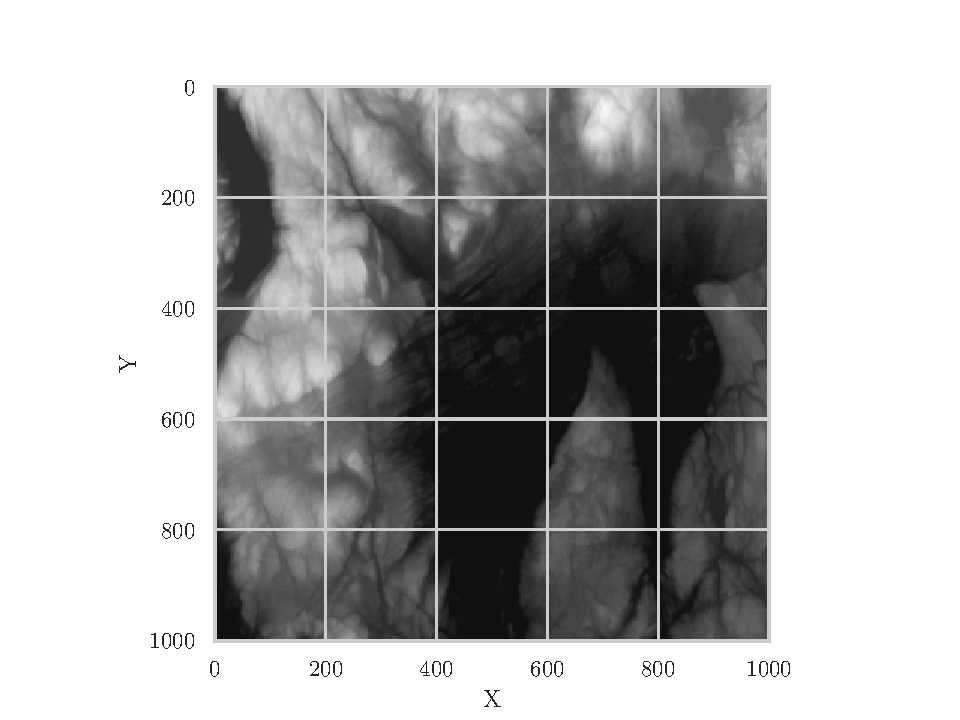
\includegraphics[width=\linewidth]{terrainpicture.pdf}
		\caption{Full terrain data over the inner \\Oslo fjord with $1000\times 1000$ data points. \\Here black represents the ocean level.}
		\label{fig:terrainpic}
	\end{subfigure}%
	\begin{subfigure}{.5\textwidth}
		\centering
		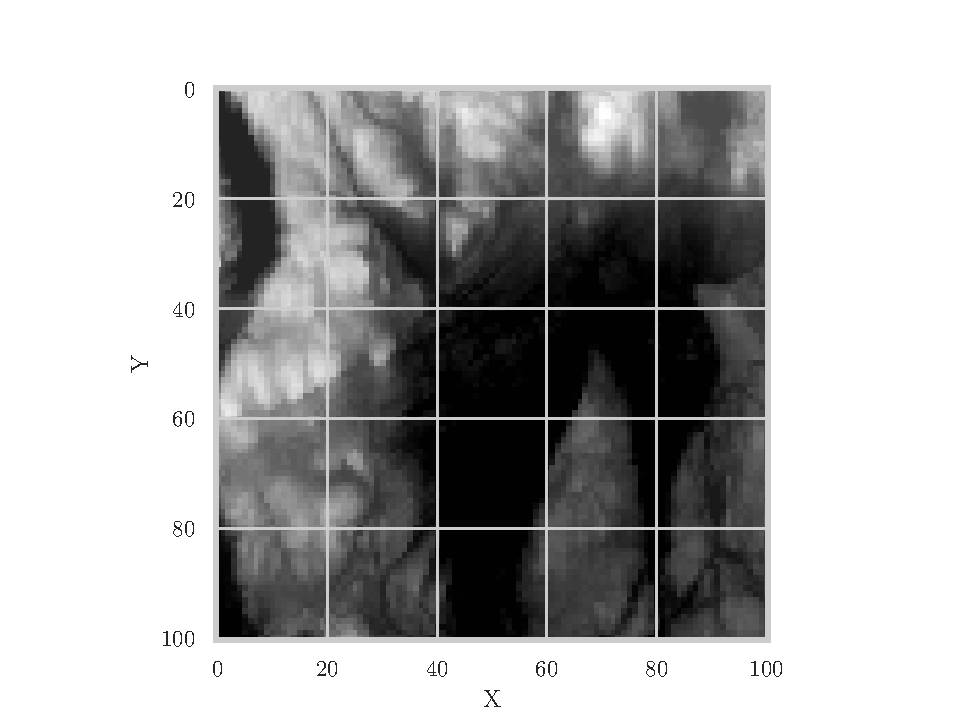
\includegraphics[width=\linewidth]{terrainpicture_reduced.pdf}
		\caption{Reduced terrain data over the inner Oslo fjord in grey scale with $100\times 100$ data points, i.e. every tenth point of every tenth row.}
	\label{fig:terrainpic_reduced}
	\end{subfigure}
	\caption{Comparison of full and reduced terrain data.}
	\label{fig:terrain}
\end{figure}

%  \[A =
%    \mqty[b_1 & c_1 & 0 & \hdots & \hdots & 0 \\
%          a_1 & b_2 & c_2 & 0 & \hdots & 0 \\
%          0 & a_2 & b_3 & c_3 & \hdots & 0 \\
%          \vdots & \ddots & \ddots & \ddots & \ddots & \vdots \\
%          0 & \hdots & \ddots & a_{n-2} & b_{n-1} & c_{n-1} \\
%          0 & \hdots & \hdots & 0 & a_{n-1} & b_n],
%  \]


\end{document}
